\documentclass[11pt]{article}
\usepackage{icamcs}


% to be able to draw some self-contained figs


%-------------------------------------------------------------------------------



%-------------------------------------------------------------------------------


%-------------------------------------------------------------------------------
\begin{document}
	%-------------------------------------------------------------------------------
	
	%don't want date printed
	\date{}
	
	% make title bold and 14 pt font (Latex default is non-bold, 16 pt)
	\title{\Large \bf Title of Contribution}
	
	%for single author (just remove % characters)
	\author{
		{\rm Your N.\ Here}\\
		Your Institution
		\and
		{\rm Second Name}\\
		Second Institution
		% copy the following lines to add more authors
		% \and
		% {\rm Name}\\
		%Name Institution
	} % end author
	
	\maketitle
	
	
	%-------------------------------------------------------------------------------
	\crule[c]{1}{1pt}
	\begin{abstract}
		%-------------------------------------------------------------------------------
		Your abstract text goes here. Your abstract text goes here. Your abstract text goes here.Your abstract text goes here. Your abstract text goes here. Your abstract text goes here.Your abstract text goes here. Your abstract text goes here. Your abstract text goes here. Your abstract text goes here. Your abstract text goes here. Your abstract text goes here.Your abstract text goes here. Your abstract text goes here. Your abstract text goes here.
	\end{abstract}
	
\vspace{0.1cm}
\textit{Keywords : }\textsf{Your keywords goes here.}
\crule[c]{1}{1pt}	
	%-------------------------------------------------------------------------------
	\section{Introduction}
	%-------------------------------------------------------------------------------
	
	A paragraph of text goes here. Lots of text. Plenty of interesting
	text. Text text text text text text text text text text text text text
	text text text text text text text text text text text text text text
	text text text text text text text text text text text text text text
	text text text text text text text.
	More fascinating text. Features galore, plethora of promises.
	
	%-------------------------------------------------------------------------------
	\section{Footnotes, Verbatim, and Citations}
	%-------------------------------------------------------------------------------
	
	Footnotes should be places after punctuation characters, without any
	spaces between said characters and footnotes, like so.%
	\footnote{ICAMCS'23.} And some embedded literal code may
	look as follows.
	\begin{theorem}
	Theorem, Theorem, Theorem, Theorem,Theorem, Theorem, Theorem, Theorem, Theorem, Theorem, Theorem, Theorem,Theorem, Theorem, Theorem, Theorem,Theorem, 
	\end{theorem}
\begin{proof}
Proof, Proof,Proof, Proof,Proof, Proof,Proof, Proof.
\end{proof}	
	Now we're going to cite somebody. Here it comes \cite{AB:2023} and \cite{ABC:2024}. Please use icamcs.bib to write your bibliography. %\cite{ABC:2024}
	

	
	%-------------------------------------------------------------------------------
	
	%-------------------------------------------------------------------------------
	
	
	%---------------------------
	
	\begin{figure}
		\begin{center}
			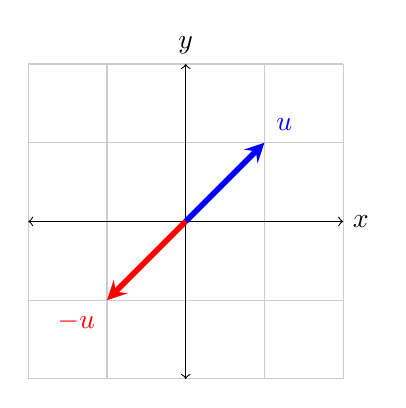
\begin{tikzpicture}
				\draw[thin,gray!40] (-2,-2) grid (2,2);
				\draw[<->] (-2,0)--(2,0) node[right]{$x$};
				\draw[<->] (0,-2)--(0,2) node[above]{$y$};
				\draw[line width=2pt,blue,-stealth](0,0)--(1,1)
				node[anchor=south west]{$\boldsymbol{u}$};
				\draw[line width=2pt,red,-stealth](0,0)--(-1,-1)
				node[anchor=north east]{$\boldsymbol{-u}$};
			\end{tikzpicture}
		\end{center}
		\caption{\label{fig:vectors}  Vectors. }
	\end{figure}
	%% %---------------------------

    \bibliographystyle{plain}
	
	\bibliography{icamcs}	

\end{document}

	